\chapter{Introduction to Organisation}\hrule
\label{Chapter:1}
% =====================================================================================================
\section {Organisation Profile and Hisotry}
I had my Six Weeks Training at Naresh I Technologies, Hyderabad. Naresh i technologies was founded in 2004 by Mr. Naresh and some of its colleagues. The company has great fame in training students in Andriod, IOS, C, C++, Java, ASP.Net, Web Technologies, Data Science related technologies across India.
\\
\\
The company main motive is to impart the deep programing and computing skills in the students across india in an affordable way. The company also provides online training on various skills like Data Science. It also have experience in training employees of various big corporate IT firms across india.\\
\\
The Institute is at 8 Km driving distance from secundrabad Junction, located in ameerpeet, Hyderabad, Telangana.It is an ISO 9001:2008 certified company. The company has a 24x7 well equipped lab facility available for its students.
\\
\\
The institute has more than 50 trainers and more than 50K students are trained in various latest software technologies in a year. The company has excellent history in software training and the company is also keenly looking forward to continue its legacy.


\chapter{Introduction to Project}\hrule
\label{Chapter:2}
% =====================================================================================================
\section{Overview}

TaxiFare aims to solve one of the biggest problems of the cab drivers that are associated with the companies like Uber, Ola etc. It can also be used by the customers using cab im order to verify that the charge taken by the driver is fair or not.\\
\\
While developing the project the main focus was that how the app will calculate a fair rate for a cab driver or user. Different API and their standard methods has been used to ensure that the app works superbly. Different latest android concepts like floating action bar also have been used in the project in order to have it a beautiful UI.\\
\\
The app will first take base rate, normal rate, rate for time as input and will calculate fare based upon distance travelled, time taken to travel the distance, base rate and normal rate as input by the user. The main challenge in the project was to calculate the distance travelled by the user. To solve the problem, i used google distance Matrix api and onLocationChanged listeners to track user co-ordinates evertime they changes their postion.\\
\\
Whenever user starts the ride, the latitude and longitude of the user is stored. When user finishes the ride the Latitude and Longitude is again stored and the distance is then calculated by using Google distance Matrix API.\\
Future of the app is very bright.It can be used as an app in between Apps like Ola, Uber and the and user. I hove the app will reach new heights in future and will solve and increase revenue for cab drivers.
\section{Existing System}

No such type of Independent App exists to calculate your Fare. Yes,there are Apps like Ola and Uber, but they work only when your book their cab.\\
In this app, you dont need to be company bounded. Hire any taxi you want and give them fair according to the deal you have done with them.
\section{User Requirement Analysis}
While hiring a private taxi, what user need is:
\begin{itemize}
	\item An input panel to enter the fair rates.
	\item Get the location and location updates automatically to calulate the distance.
	\item Get the correct distance travelled.
	\item Get the correct time taken to travel the distance.
	\item Fair should be calculated fairly on the end of the ride
	\item Fair details should be shown after the ride ends.
\end{itemize}

\section{Feasibility Study}
The application is fully feasible. It just needs a working internet connection,a gps and android 4.0 and above. It is fully feasible if it is also deployed on a large scale.\\
The application can also be upgraded further and can be deployed on large scale depending upon the need of business plan.\\
It can also be integrated with other taxi apps using API of other apps in the App.\\
The application is fully feasible according to the current needs of user and also feasible with the development cost.
\section{Objectives of the Project }
\begin{itemize}
	\item The project was developed to give a solution to the taxi customers.
	\item The main motive behind developing the project was to provide a fair method to pay for a ride in a taxi or private auto based upon distance travelled and time taken to travel the distance.
	\item App can be used by taxi drivers of various companies like Ola, Uber when they are free and can have cutomers instead of sitting idle.
\end{itemize}


\chapter{Product Design}\hrule
\label{Chapter:3}
% =====================================================================================================

\section{Product Perspective}
The application will have a user friendly and menu based interface.Following screens will be provided:
\begin{itemize}
	\item A google map actvity screen.
	\item Two floating action buttons.
	\item Left FAB to set fare and Right FAB to get current. location
	\item There are two more buttons,one to BOOK RIDE and other to end Ride.
	\item One alert dialogue will be generated after end of ride.
	\item Alert dialogue will have fare details like time taken, distance travelled and total fare.
\end{itemize}
\section{Product Functions}
\begin{itemize}
	\item User can input base rate and rate manually
	\item User just need to click start ride when they start their journey
	\item User needs to click end ride when he/she completes the journey
	\item App will calculate distance travelled by user automatically
	\item App will calculate time taken by user to travel the distance automatically
	\item App will automatically calculate Fare for the journey.\\
\end{itemize}
\section{User characteristics}
User will get a flaoting action button. After clicking left FAB, user will have to input rate and base rate.\\
User needs to click start ride and end ride buttons, rest all will be taken care by the app.
\section{Constraints} 
\begin{itemize}
	\item User needs Android 4.0 and above.
	\item User needs active internet connection and gps connection.
	\item User have to set fare and base fare rate at the time of starting the app, just once.
	\item Rates will be saved untill it is overridden.
\end{itemize}
\section{Flow Chart}
\begin{figure}[h]
\centering
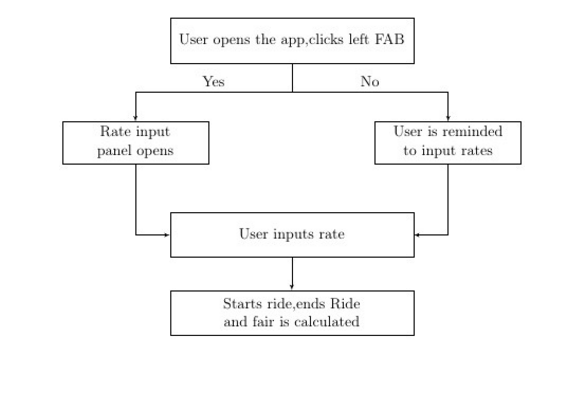
\includegraphics[width=0.75\linewidth]{p01}
\caption{Control flow diagram}
\label{fig:p01}
\end{figure}
When user opens the app,does he clicks the left floating action bar?\\
If yes, he is directed to input the rate.If no, user is reminded to input the rate.\\
User inputs the rate, then he is directed back to the main activity.\\
He books the ride, ends the ride and the fair is calculated.

\section{Assumptions and Dependencies}
\begin{itemize}
	\item User is assumed to be using Android 4.0 and above.
	\item User is assumed to have working internet and gps connection.
	\item Fair is dependent on the base rate and rate entered by the user.
	\item Fair is also dependent on the distance travelled  and time taken to travel the distance. 
	\item Time travel calculation is dependent on the system time.
\end{itemize}
\section{Specific Requirements}
\begin{itemize}
	\item Android 4.0 and above.
	\item Working internet connection.
	\item Working gps connection.
\end{itemize}
\chapter{Development and Implementation}\hrule
\label{Chapter:4}
% =====================================================================================================
\section{Introduction to Languages}
\subsection{Front End}
XML is used as to design beautiful UI to give user a beautiful experience. Now a days, an app business is more dependent on how interactive, beautiful and simple your UI is.\\
\\
The Android platform is an open source mobile development platform. It gives you access to all aspects of the mobile device that it runs on, from low level graphics, to hardware like the camera on a phone. With so many things possible using Android, you might wonder why you need to bother with XML. It is not that working with XML is so interesting, it is working with the things that it enables. XML is commonly used as a data format on the Internet. If you want to access data from the Internet, chances are that the data will be in the form of XML. If you want to send data to a Web service, you might also need to send XML. In short, if your Android application will leverage the Internet, then you will probably need to work with XML. Luckily, you have a lot of options available for working with XML on Android.
\subsection{Back End}
In the back end,JAVA is used. Collection and Genrics concepts are mainly used. Java is one of the world's most important and widely used computer languages, and it has held this distinction for many years. Unlike some other computer languages whose influence has weared with passage of time, while Java's has grown.\\

As of 2016, Java is one of the most popular programming languages in use, particularly for client-server web applications, with a reported 11 million developers using and working on it.\\

Applications of java:\\
Java is widely used in every corner of world and of human life. Java is not only used in softwares but is also widely used in designing hardware controlling software components. There are more than 930 million JRE downloads each year and 3 billion mobile phones run java.

Following are some other usage of Java :
\begin{itemize}
	\item Developing Desktop Applications.
	\item Web Applications like Linkedin.com, Snapdeal.com etc.
    \item	Mobile Operating System like Android.
    \item	Embedded Systems.
	\item Robotics and games etc.
\end{itemize}

\section{Supporting Languages}
Follwing API are used:
\begin{itemize}
	\item Google Maps API for Android.
	\item Google places API for Android.
	\item Google distance Matrix API.
\end{itemize}
Along with these API, some inbuilt methods of android sdk and Java are also used.
\section{Implementation with ScreenShots}
	First the main activity opens,there we have two floating action bars, one button to start ride.After clicking on the left FAB,rate activity opens, which is as follows:
\begin{figure}[h]
	\centering
	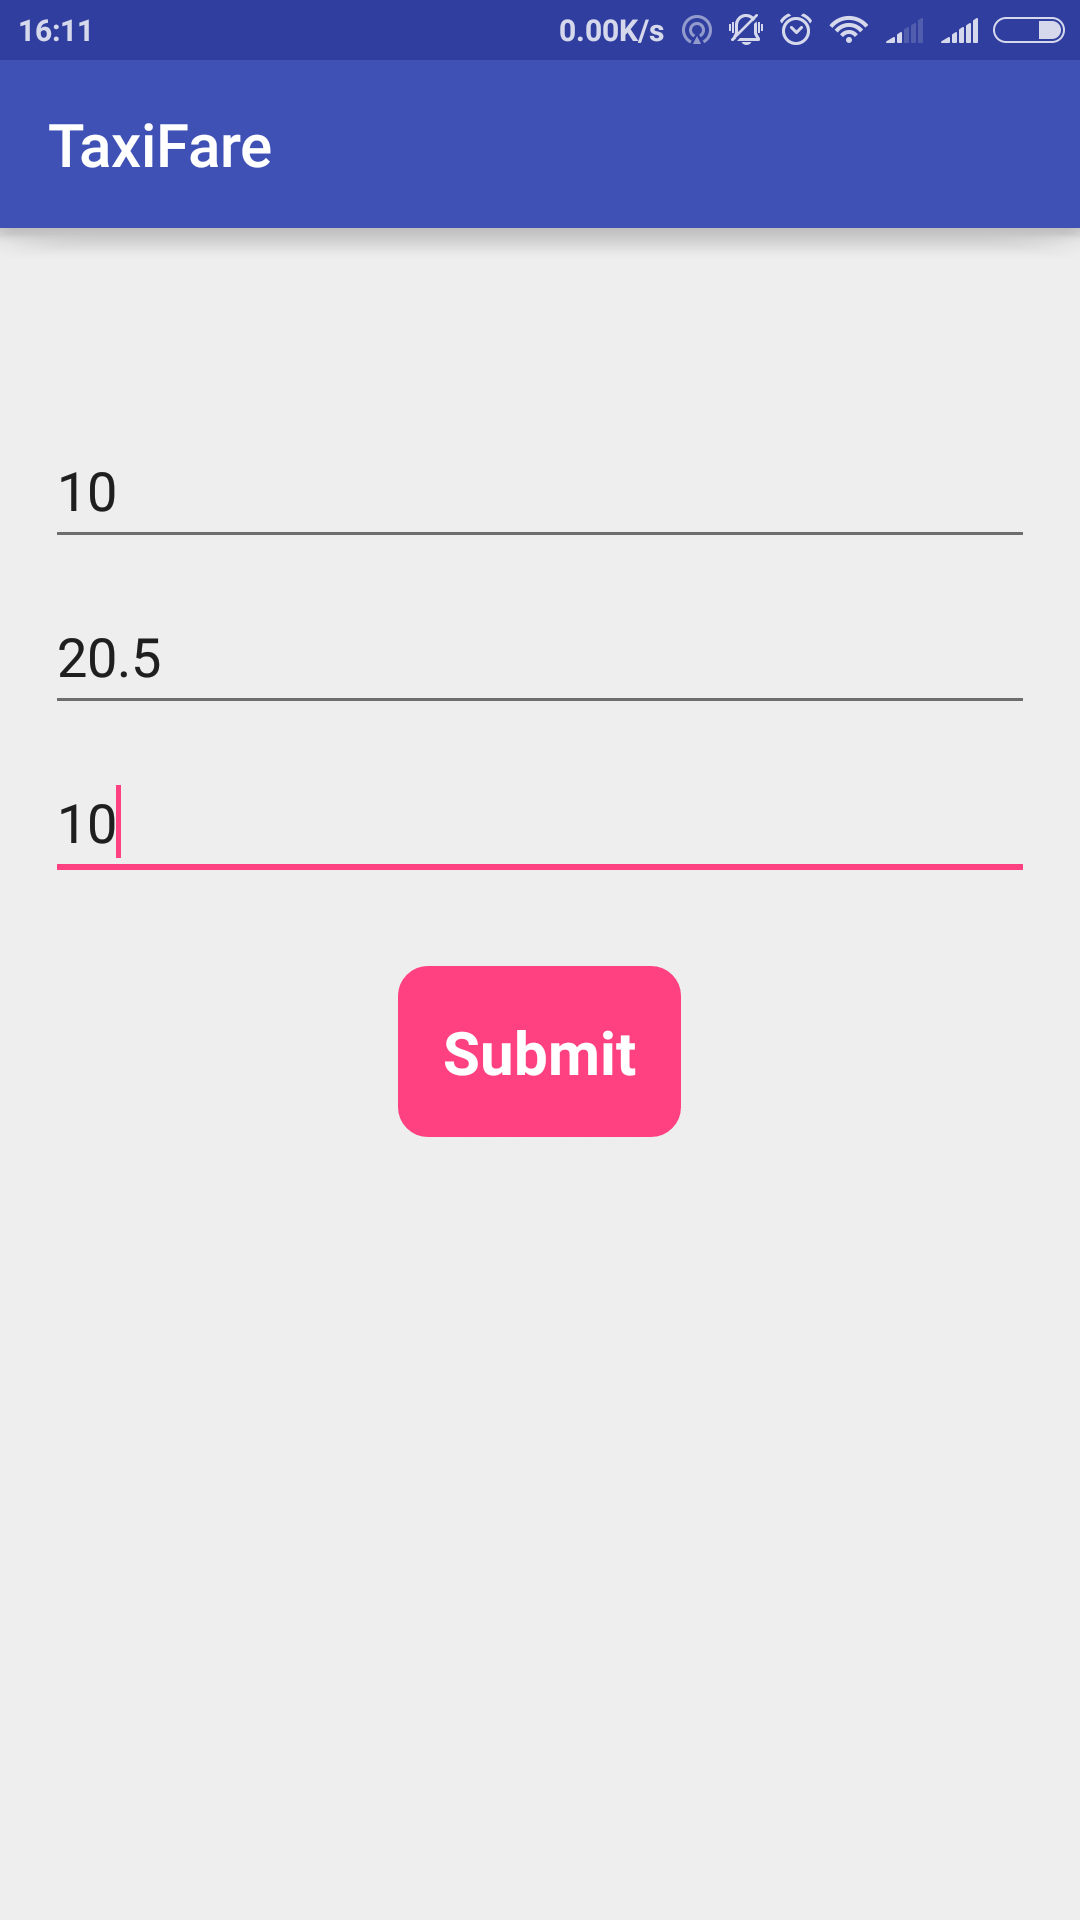
\includegraphics[width=0.7\linewidth]{p05}
	\caption{Rate Activity}
\end{figure}
\\
After entering the rates,MapsActivity opens. Here you will see a start ride button. Click on start ride button to start ride.

\begin{figure}[h]
\centering
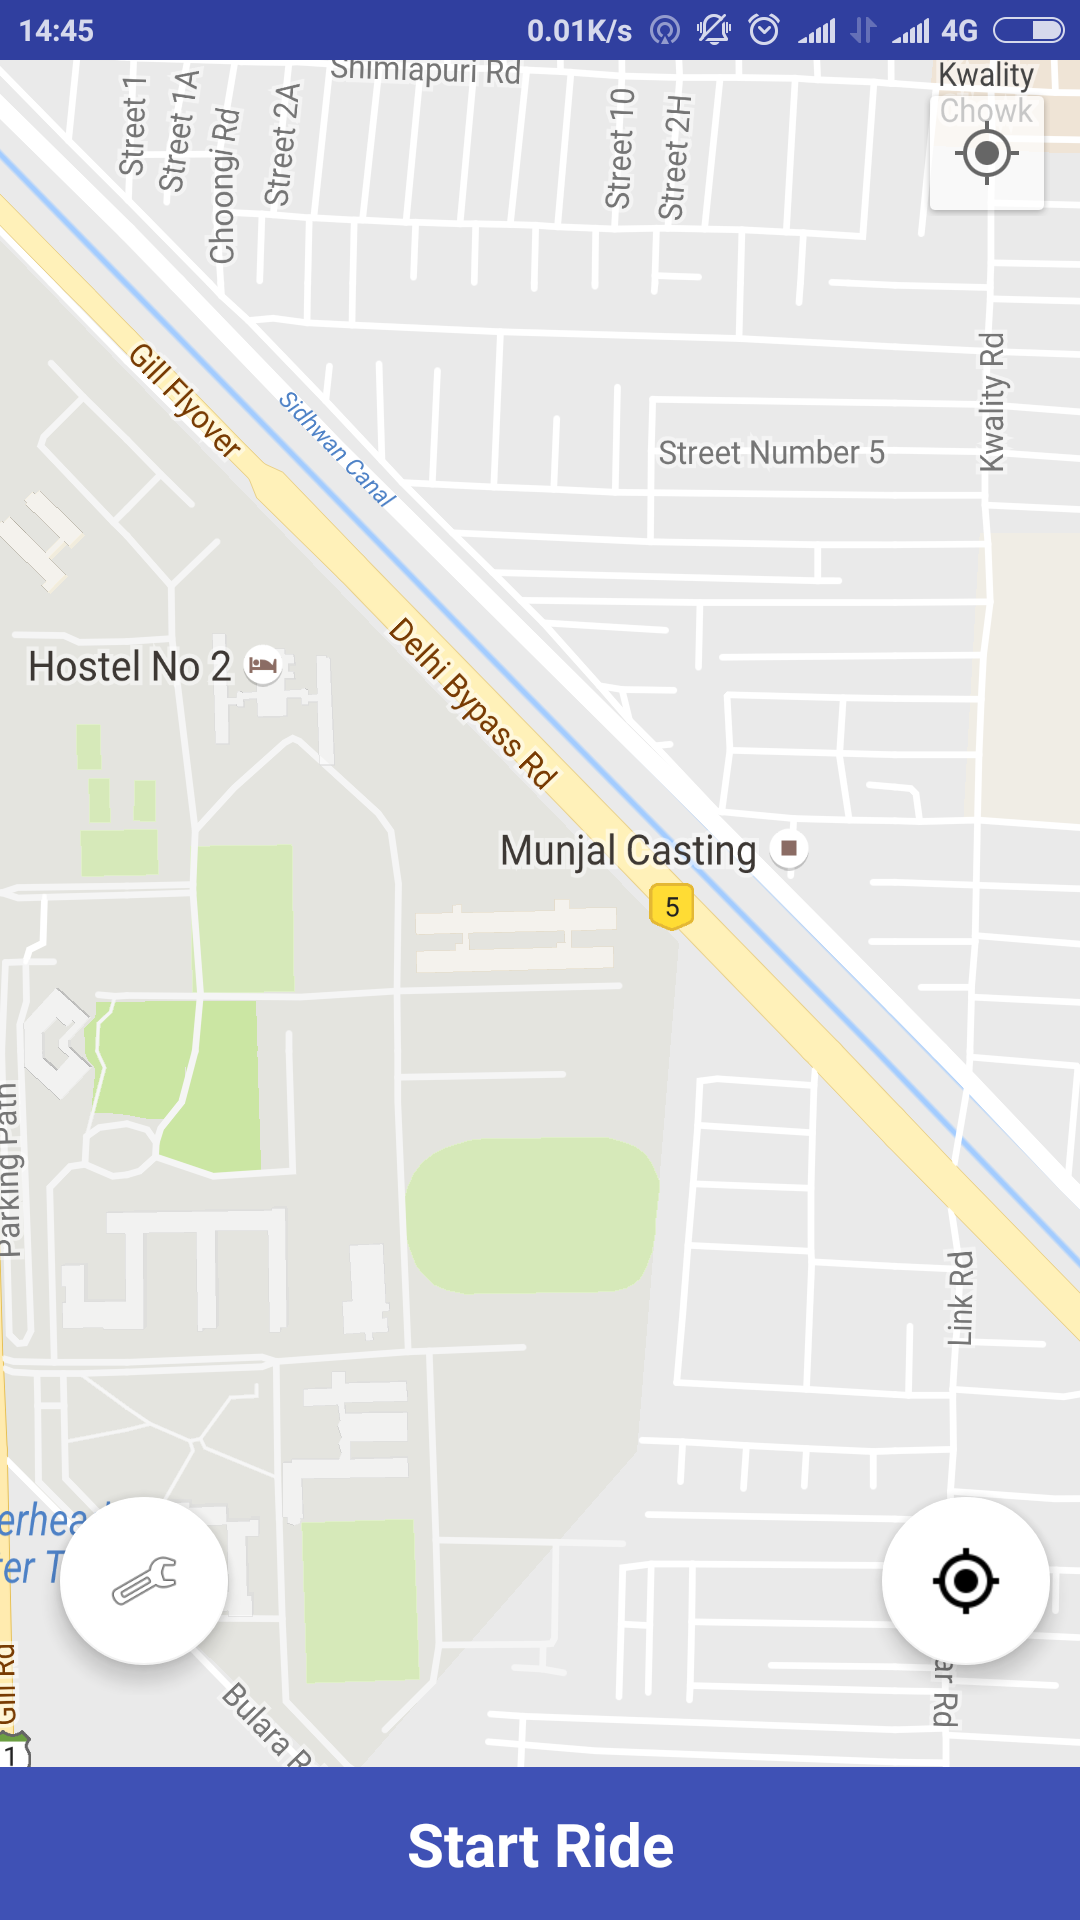
\includegraphics[width=0.7\linewidth]{p03}
\caption{Start Ride activity}
\end{figure}
\begin{text}
	\\
	\\
\end{text}	
After starting the ride, End ride button is visible now. When you have reached your destination, click on end ride button to finish your ride.
\begin{figure}[h]
	\centering
	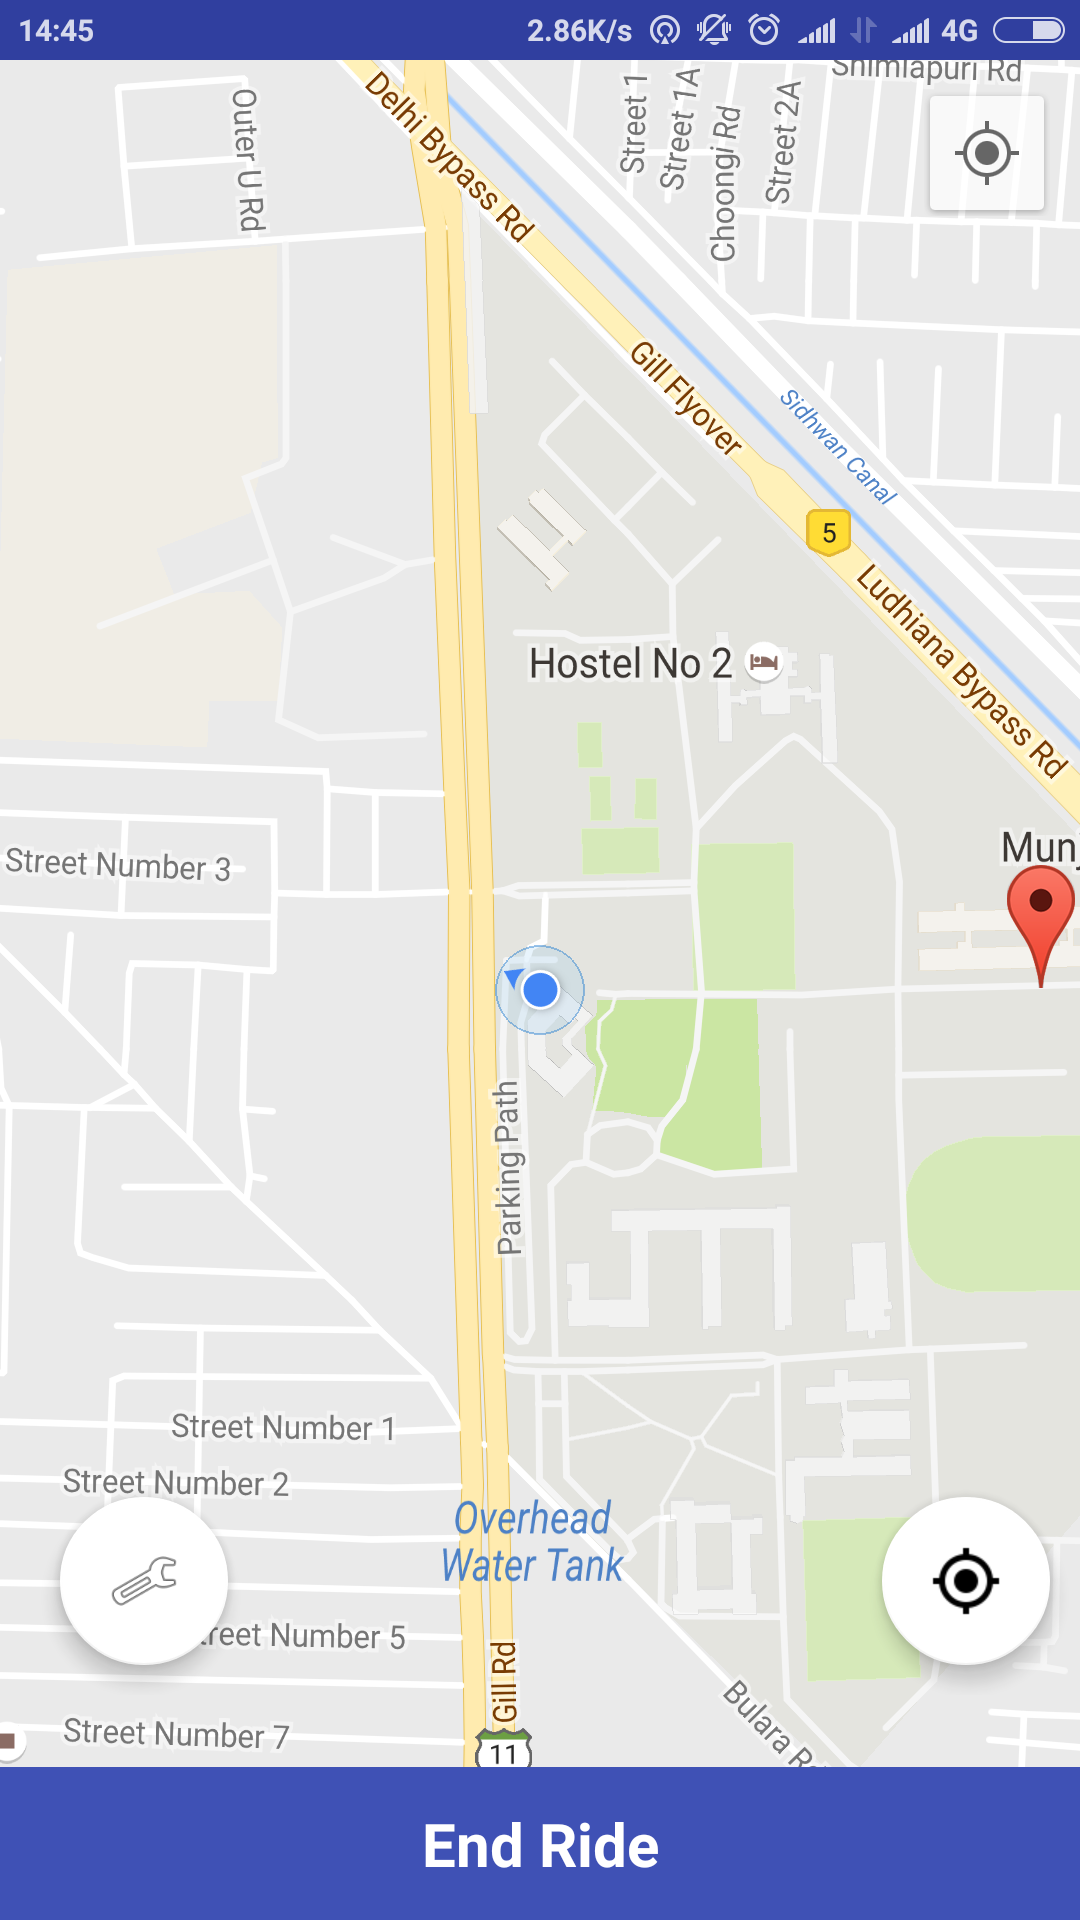
\includegraphics[width=0.7\linewidth]{p04}
	\caption{End Ride activity}
\end{figure}
\\
After the End ride button is clicked, A dialogue box appears showing fare deatils like distance travelled, time taken and total fare.
\begin{figure}[h]
	\centering
	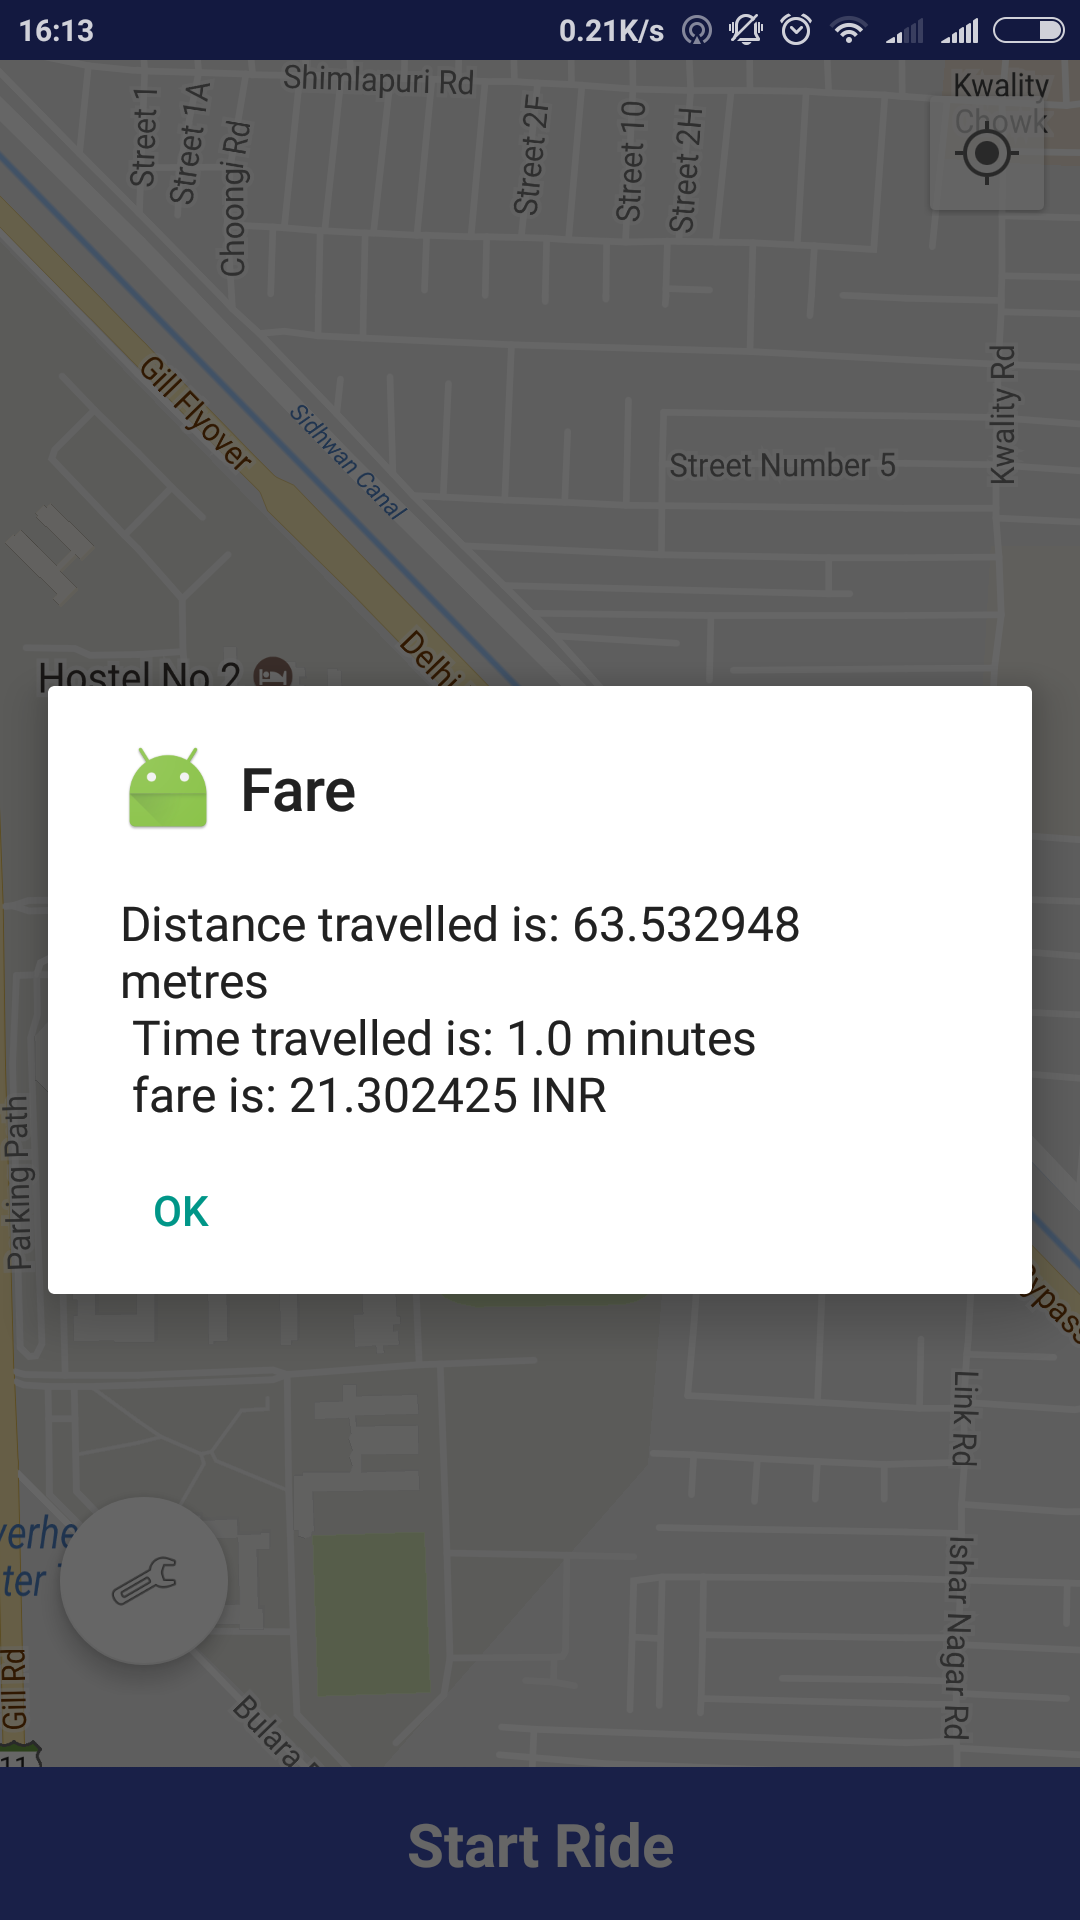
\includegraphics[width=0.7\linewidth]{p02}
	\caption{Fair Shown by dialogue box}
\end{figure}


\section{Testing}
Software testing is a critical element of the ultimate review of specification design and coding. Testing of software leads to the uncovering of errors in the software functional and
performance requirements are met. Testing also provides a good indication of software reliability and software quality as a whole. The result of different phases of testing are evaluated and then compared with the expected results. If the errors are uncovered they are debugged and corrected. A strategy approach to software testing has the generic characteristics:
\begin{itemize}
	\item Testing begins at the module level and works outwards towards the integration of
	the entire computer based system.
	\item Testing and debugging are different activities, but debugging must be accommodated in the testing strategy.
	\item Different testing techniques are appropriate at different points of time.
\end{itemize}
Testing of the app is done by JUnit tester providev inbuilt in the android studio.
\\
The app is also tested in realtime environment.It has passed all the tests conducted by Junit and in realtime sucessfully.
\\
The app has also been tested on custom user inputs.
\chapter{Conclusion and Future Scope}\hrule
\label{Chapter:5}
% =====================================================================================================
\section{Conclusion}
The product which we developed was implemented and tested with data and were found to be error free. Also, it is found that the product will work successfully. We tried to make the product maximum user friendly. All the necessary validations are carried out in this project, so that any kind of users can make use of this product and a necessary message makes them conscious of the error they have made. This product is developed
with scalability in mind. Additional modules can be easily added when necessary. The software is developed with modular approach. All modules in this system have been tested separately and put together to form the main system. Finally the system is tested with data and everything worked successfully.
\section{Future Scope}
The app has been developed keeping in future of the different Taxi apps.\\
Different taxi API's can be used and mashed up together to develop an App which will help Driver to get bookings in their free time and increase their revenue.\\
The App has main moto to increase revenue of drivers and make them earn money more in less time. I hope,the App will achieve its aim of development and will generate a great revenue for developer and driver.
\chapter{Refrences}\hrule
\label{Chapter:6}
% =====================================================================================================
\begin{enumerate}
	\item http://www.vogella.com/tutorials/android.html [accesed on 14/06/2016].
	\item https://www.tutorialspoint.com/android/ [accesed on 21/06/2016].
	\item https://developers.google.com/maps/documentation/android-api/marker [accesed on 02/07/2016].
	\item http://www.javatpoint.com/android-tutorial [accesed on 05/07/2016]
	\item http://www.vogella.com/tutorials/AndroidGoogleMaps/article.html [accesed on \\10/07/2016].
	\item http://android-developers.blogspot.in/search?updated-min=\\2016-01-01T00:00:00-08:00updated-max=2017-01-01T00:00:00-08:00max-results=50 [accesed on 12/07/2016].
\end{enumerate}